%%%%%%%%%%%%%%%%%%%%%%%%%%%%%%%%%%%%%%%%%
% Structured General Purpose Assignment
% LaTeX Template
%
% This template has been downloaded from:
% http://www.latextemplates.com
%
% Original author:
%  Ted Pavlic (http://www.tedpavlic.com)
% Modified by:
%  Joe Del Rocco (https://joe.delrocco.org)
%%%%%%%%%%%%%%%%%%%%%%%%%%%%%%%%%%%%%%%%%

%----------------------------------------------------------------------------------------
%  PACKAGES AND CONFIGURATION
%----------------------------------------------------------------------------------------

\documentclass[fleqn]{article}
\usepackage{geometry}
\usepackage{fancyhdr} % For custom headers
\usepackage{lastpage} % To determine the last page for the footer
\usepackage{extramarks} % For headers and footers
\usepackage[most]{tcolorbox} % For Question answer sections
\usepackage{graphicx} % For inserting images
\usepackage{xcolor} % For link coloring
\usepackage[hidelinks]{hyperref} % For URL links (no box or color name)

% Margins
\geometry{
a4paper,
tmargin=1in,
bmargin=1in,
lmargin=1in,
rmargin=1in,
textwidth=6.5in,
textheight=9.0in,
headsep=0.25in
}

% Header and footer
\pagestyle{fancy}
\lhead{\myName} % Top left header
\chead{\myCourse: \myAssignment} % Top center header
\rhead{\firstxmark} % Top right header
\lfoot{\lastxmark} % Bottom left footer
\cfoot{} % Bottom center footer
\rfoot{Page\ \thepage\ of\ \pageref{LastPage}} % Bottom right footer
\renewcommand\headrulewidth{0.4pt} % Size of the header rule
\renewcommand\footrulewidth{0.4pt} % Size of the footer rule

% Other configurations
\setlength\parindent{0pt} % Removes all indentation from paragraphs
\setlength\parskip{1pt} % Ensures paragraphs are still recognizable as such
\setcounter{secnumdepth}{0} % Removes default section numbers
\setcounter{tocdepth}{3} % Sets depth of table of contents
\linespread{1.1}

% Template values
\newcommand{\myName}{Ayush Tiwari, Udit Desai}
\newcommand{\myEmail}{ayushtiwari@icloud.com}
\newcommand{\myCourse}{CS39006}
\newcommand{\mySection}{Spring 2020}
\newcommand{\myTeacher}{RSC}
\newcommand{\myAssignment}{Assignment~1}

%----------------------------------------------------------------------------------------
%  DOCUMENT STRUCTURE (MACROS & ENVIRONMENTS)
%----------------------------------------------------------------------------------------

% Colored links macro
\newcommand{\hrefcol}[3] {\href{#1}{\textcolor{#3}{#2}}}

% Creates a counter to keep track of the number of Questions
\newcounter{homeworkQuestionCounter}

% Macro for custom title page signature header
\newsavebox{\myTitleSignature}
\sbox{\myTitleSignature}{%
\begin{tabular*}{\textwidth}{@{}l@{}@{\extracolsep{0.125in}}l@{}}%
\parbox{4.25in}{\raggedright{}} &
\parbox[c][]{2.5in}{{\textbf{\myName} \par}
                    {\small 17CS10056, 17CS30044 \par}
                    {\small \hrefcol{mailto:\myEmail}{}{blue}} \par}
\end{tabular*}}

% Header and footer for when a page split occurs within a Question environment
\newcommand{\enterQuestionHeader}[1]{%
\nobreak\extramarks{#1}{#1 continued on next page\ldots}\nobreak%
\nobreak\extramarks{#1 (continued)}{#1 continued on next page\ldots}\nobreak%
}

% Header and footer for when a page split occurs between Question environments
\newcommand{\exitQuestionHeader}[1]{%
\nobreak\extramarks{#1 (continued)}{#1 continued on next page\ldots}\nobreak%
\nobreak\extramarks{#1}{}\nobreak%
}

\newcommand{\homeworkQuestionName}{} % Argument = name of Question; default = "Question #"
\newenvironment{homeworkQuestion}[1][Question \arabic{homeworkQuestionCounter}]{%
\stepcounter{homeworkQuestionCounter}% % Increase counter for number of Questions
\renewcommand{\homeworkQuestionName}{#1}% % Assign \homeworkQuestionName the argument
\section{\homeworkQuestionName}% % Make a section in the document with the custom Question count
\enterQuestionHeader{\homeworkQuestionName}% % Header and footer within environment
}{%
\exitQuestionHeader{\homeworkQuestionName}% % Header and footer after environment
}

\newcommand{\QuestionAnswer}[1]{ % Defines the Question answer command with the content as the only argument
\begin{tcolorbox}[breakable,enhanced,colback=gray!5!white,title=Answer]%
#1
\end{tcolorbox}%
% Alternative - Makes the box around the Question answer and puts the content inside
%\noindent\framebox[\columnwidth][c]{\begin{minipage}{0.98\columnwidth}#1\end{minipage}}
}

\newcommand{\homeworkSectionName}{}
\newenvironment{homeworkSection}[1]{% % For sections w/in Questions; Argument = name of section (no default)
\renewcommand{\homeworkSectionName}{#1}% % Assign \homeworkSectionName the argument
\subsection{\homeworkSectionName}% % Make a subsection with the name of the subsection
\enterQuestionHeader{\homeworkQuestionName\ [\homeworkSectionName]}% % Header and footer within environment
}{%
\enterQuestionHeader{\homeworkQuestionName}% % Header and footer after environment
}

%----------------------------------------------------------------------------------------
%   TITLE PAGE
%----------------------------------------------------------------------------------------
\begin{document}

% Blank out the traditional title page
\title{\vspace{-1in}} % no title name
\author{} % no author name
\date{} % no date listed
\maketitle % makes this a title page

% Use custom title macro instead
\usebox{\myTitleSignature}
\vspace{1in} % spacing below title header

% Assignment title
{\centering \huge \myAssignment \par}
{\centering \noindent\rule{4in}{0.1pt} \par}
\vspace{0.05in}
{\centering \myCourse~: \mySection \par}
{\centering Date : 16/01/2020 \par}
%{\centering Prepared w/ \LaTeX \par}
\vspace{1in}

% Table of Contents
\tableofcontents
\vspace{170pt}
\textbf{Note 1 :}\textit{ The key steps involve setting the \textbf{filters} and executing \textbf{commands} on terminal. These have been mentioned at the beginning of each answer as and where necessary.} \par
\textbf{Note 2 :}\textit{ Justifications are written in italics.}
\newpage

%----------------------------------------------------------------------------------------
%	Question 1
%----------------------------------------------------------------------------------------

%\begin{homeworkQuestion}[Exercise \#\arabic{homeworkQuestionCounter}] % Use for custom section title
\begin{homeworkQuestion}
List the different protocols that you observe in the packet trace, at application, transport and network layer for each of the UDP and TCP test cases.\par
\vspace{10pt}

\QuestionAnswer{
\textbf{\large TCP} \par
\vspace{5pt}
{\textsf Command : \ttfamily wget --no-proxy http://10.5.18.163:8000/1.jpg } \par
\vspace{5pt}
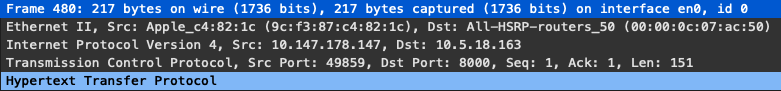
\includegraphics[scale=0.45]{tcp_protocols_2.png} \par
\vspace{5pt}
1. Application Layer : HTTP \par
2. Transport Layer : TCP \par
3. Network Layer : IPv4 \par
\vspace{5pt}
\textit{wget is an application layer tool for sending HTTP requests.}\par
\vspace{10pt}
\textbf{\large UDP} \par
\vspace{5pt}
{\textsf Command : \ttfamily iperf3 -c 10.5.18.163 -u -b 28000 } \par
\vspace{5pt}
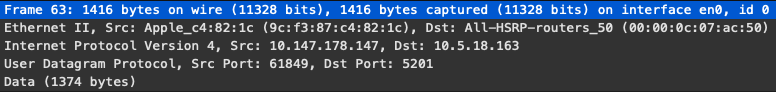
\includegraphics[scale=0.45]{udp_protocols.png} \par
\vspace{5pt}
1. Transport Layer : UDP\par
2. Network Layer : IPv4 \par
\vspace{5pt}
\textit{iperf is a transport layer tool and -u flag is used to send UDP packets.}
}




\end{homeworkQuestion}

%----------------------------------------------------------------------------------------
%	Question 2
%----------------------------------------------------------------------------------------

\begin{homeworkQuestion}
Analyse the packet trace using Wireshark and compute the following: \par

%-----------------------------------------------

\begin{homeworkSection}{(a)}
How many TCP packets are transferred for each cases while accessing the files 1.jpg to 5.jpg ? Are all packets of same size? What are the different packet size you observe for each of the file access?
\vspace{10pt}

\QuestionAnswer{
\textsf{Filters} : \textbf{ip.addr==10.5.18.163 \&\& ip.addr==client\textunderscore ip} \par
\vspace{10pt}
\textbf{\large \underline{Screenshots of Packet Lengths}} \par
\vspace{5pt}
Count value of the first row shows the total no. of packets. \par
\vspace{10pt}
\textbf{\small 1.jpg} \par
\vspace{10pt}
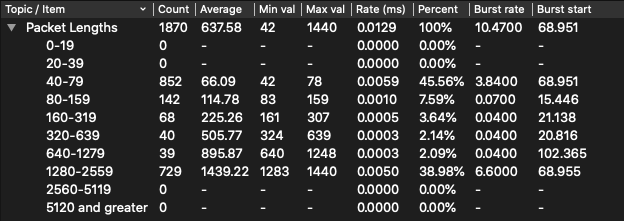
\includegraphics[scale=0.5]{packets_1.png} \par
\vspace{10pt}
\textbf{\small 2.jpg} \par
\vspace{10pt}
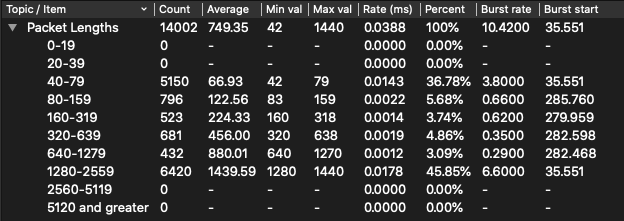
\includegraphics[scale=0.5]{packets_2.png} \par
\vspace{10pt}
\textbf{\small 3.jpg} \par
\vspace{10pt}
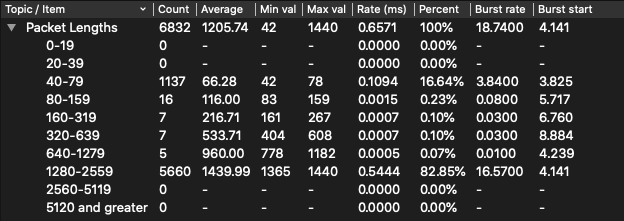
\includegraphics[scale=0.5]{packets_3.png} \par
\vspace{10pt}
\textbf{\small 4.jpg} \par
\vspace{10pt}
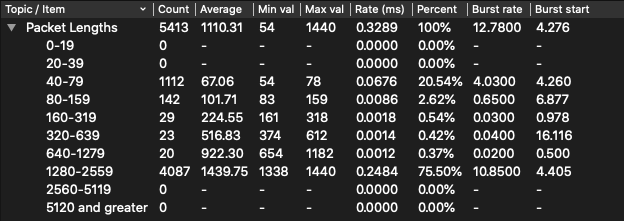
\includegraphics[scale=0.5]{packets_4.png} \par
\vspace{10pt}
\textbf{\small 5.jpg} \par
\vspace{10pt}
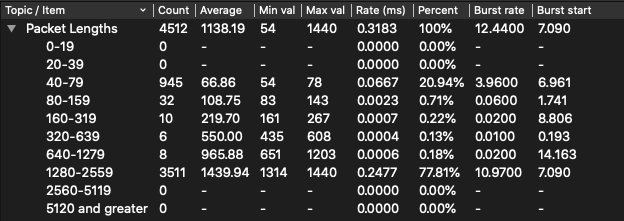
\includegraphics[scale=0.5]{packets_5.png} \par
\vspace{10pt}
\textbf{\large \underline{Justification}} \par
\vspace{5pt}
\textit{1. Since the pictures are of different sizes and downloaded using a TCP protocol, number of data packets are different in all the cases.} \par
\vspace{5pt}
\textit{2. All the packets are not of the same size and there were various sizes ranging from 45 to a few thousands. Generally, the ACK packets are of less size compared to the data packets.}
}
\end{homeworkSection}

%-----------------------------------------------

\begin{homeworkSection}{(b)}
For the test case with UDP, are all the UDP packets of the same size? If not, what are the different UDP packet sizes you observe?
\vspace{10pt}

\QuestionAnswer{
All packets are of the same size i.e. $1416$
}
\end{homeworkSection}

\begin{homeworkSection}{(c)}
Observe the TCP and UDP throughput using Wireshark (Menu - Statistics - IO Graphs)
\vspace{10pt}

\QuestionAnswer{
\textbf{\small TCP} \par
\vspace{10pt}
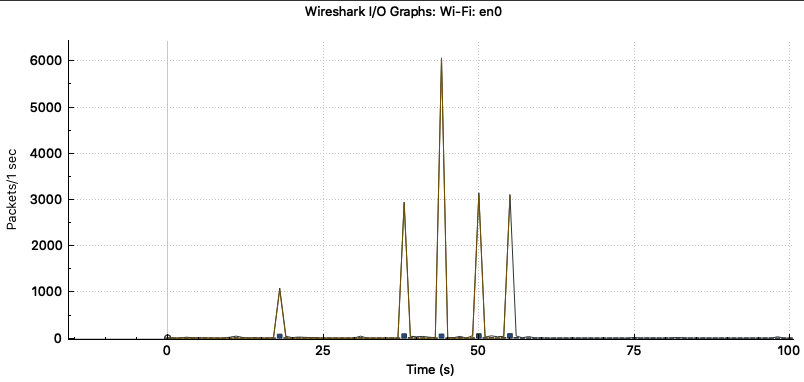
\includegraphics[scale=0.5]{tcp_throughput.png} \par
\vspace{5pt}
\textit{5 elevations in the graphs corresponds to 5 pictures transferred from server to client. Since each picture is requested only after receiving the previous picture each peak corresponds to one picture.} \par
\vspace{10pt}
\textbf{\small UDP} \par
\vspace{10pt}
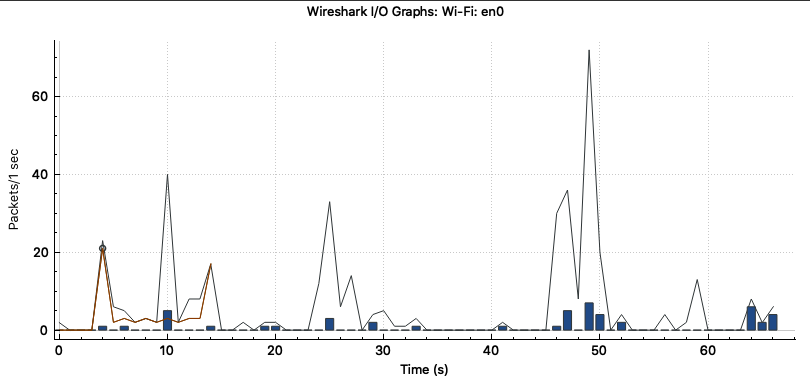
\includegraphics[scale=0.5]{udp_graph.png} \par
}
\end{homeworkSection}

\begin{homeworkSection}{(d)}
Compute the UDP throughput (amount of UDP data sent per second) for following cases of UDP traffic generation rates (bandwidth): \par
(i) 64 Kbps (ii) 128 Kbps (iii) 256 Kbps (iv) 512 Kbps (v) 1024 Kbps (vi) 2048 Kbps
\vspace{10pt}

\QuestionAnswer{
{\textsf Command : \ttfamily iperf3 -c 10.5.18.163 -u -b 28000 } \par
{\textsf Filters : \textbf{ip.addr==10.5.18.163 \&\& ip.addr==client\textunderscore ip \&\& udp} } \par
\vspace{10pt}
\large{Sample Output on Terminal} \par
\vspace{5pt}
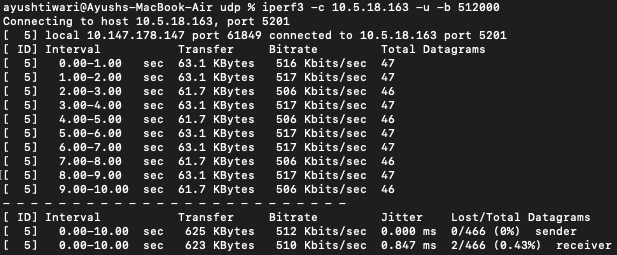
\includegraphics[scale=0.5]{sample.png} \par
\vspace{10pt}
\textbf{ \large \underline{Observations}} \par
\vspace{10pt}
\textbf{\small i) $64$Kbps} \par
\vspace{10pt}
Data Sent : $83544$\par
No. of Packets : $59$\par
Time taken : $9.9588$s\par
Throughput : $8388$Kbps\par
\vspace{10pt}
\textbf{\small ii) $128$Kbps} \par
\vspace{10pt}
Data Sent : $165672$\par
No. of Packets : $117$\par
Time taken : $9.9598$s\par
Throughput : $16634$Kbps\par
\vspace{10pt}
\textbf{\small iii) $256$Kbps} \par
\vspace{10pt}
Data Sent : $329928$\par
No. of Packets : $233$\par
Time taken : $9.9610$s\par
Throughput : $33121$Kbps\par
\vspace{10pt}
\textbf{\small iv) $512$Kbps} \par
\vspace{10pt}
Data Sent : $659856$\par
No. of Packets : $466$\par
Time taken : $9.9619$s\par
Throughput : $66237$Kbps\par
\vspace{10pt}
\textbf{\small v) $1024$Kbps} \par
\vspace{10pt}
Data Sent : $1318296$\par
No. of Packets : $931$\par
Time taken : $9.9630$s\par
Throughput : $132319$Kbps\par
\vspace{10pt}
\textbf{\small vi) $2048$Kbps} \par
\vspace{10pt}
Data Sent : $2636592$\par
No. of Packets : $1862$\par
Time taken : $9.9641$s\par
Throughput : $264609$Kbps\par
\vspace{10pt}
}
\end{homeworkSection}


\end{homeworkQuestion}

%----------------------------------------------------------------------------------------
%	Question 3
%----------------------------------------------------------------------------------------

\begin{homeworkQuestion}
Analyze the number of TCP packets retransmitted (Use: tcp.analysis.retransmission filter.) from Wireshark. \par
\vspace{10pt}

\QuestionAnswer{
\textsf{Filters} : \textbf{ip.addr==10.5.18.163 \&\& ip.addr==client\textunderscore ip \&\& tcp.analysis.retransmission} \par
\vspace{5pt}
Observed number of TCP packets retransmitted : $0$ \par
\vspace{5pt}
\textit{Number of retransmissions packets lost will depend on strength and traffic of the network connection.}
}
\end{homeworkQuestion}

\begin{homeworkQuestion}
Plot the following: \par

%-----------------------------------------------

\begin{homeworkSection}{(a)}
UDP throughput with respect to the UDP bandwidth.
\vspace{10pt}

\QuestionAnswer{
\textbf{\small i) x-axis : Bandwidth (Kbps)} \par
\textbf{\small i) y-axis : Throughput (Kbps)} \par
\vspace{10pt}
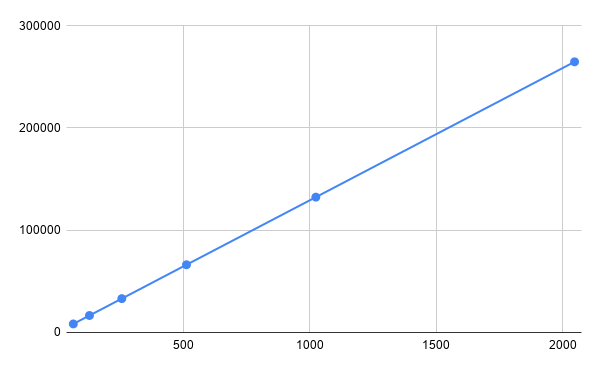
\includegraphics[scale=0.65]{throughput_bandwidth.png} \par
}
\end{homeworkSection}

%-----------------------------------------------

\begin{homeworkSection}{(b)}
Number of UDP packets transmitted with respect to UDP bandwidth.
\vspace{10pt}
\newpage
\QuestionAnswer{
\textbf{\small i) x-axis : Bandwidth (Kbps)} \par
\textbf{\small i) y-axis : No of packets } \par
\vspace{10pt}
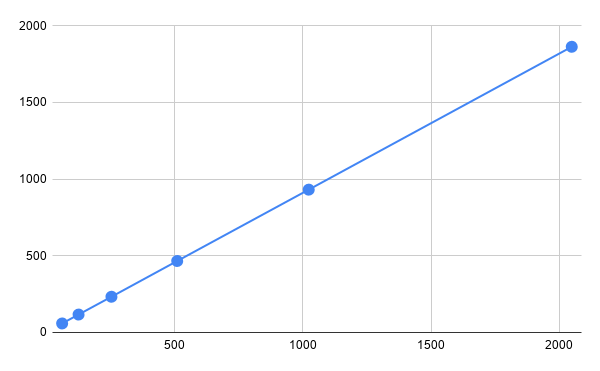
\includegraphics[scale=0.65]{no_of_packets_bandwidth.png} \par
}
\end{homeworkSection}
\vspace{10pt}
What are your observations from these plots? \par
\vspace{10pt}
\QuestionAnswer{
As \textbf{bandwidth} increases, the number of packets being transferred in the same time (about {\large 10s}) and throughput also increase. The relationship observed is linear.
}

\end{homeworkQuestion}

\end{document}
%----------------------------------------------------------------------------------------
%	DONE
%----------------------------------------------------------------------------------------
